\newpage
\section{Suggested solutions: Discrete-time Signals}
\begin{enumerate}
\item The signal $x(t)=Ae^{i\omega_{0}t}$ is discretized using an ideal continuous-to-discrete time converter $x[n]=x(nT_{s})=Ae^{i\hat{\omega}_{k}n}$. Let $A=1$ and $\omega_{0}=2\pi 10042$ rad/s. Let the sample rate be $f_{s}=100$ samples per second and $T_{s}=1/f_{s}$.

\begin{enumerate}[a)]
\item Have $\hat{\omega}_{0}=\omega_{0}T_{s}$ and $\hat{\omega}_{k}$ is
$$\hat{\omega}_{k}=\hat{\omega}_{0}+2\pi k=\omega_{0}\frac{1}{f_{s}}+2\pi k=\frac{5021}{25}\pi+2\pi k$$
for $k\in\mathbb{Z}$. 

\item The principal aliases lie in $-\pi<\hat{\omega}_{k}<\pi$. Pick a $k\in\mathbb{Z}$ such that $-\pi<\hat{\omega}_{k}<\pi$. For instance $k=100$ works:
$$-\pi < \frac{5021}{25}\pi-2\pi 100 < \pi,$$
giving a value of $\hat{\omega}\approx2.6389\ \text{rad/sample}$. 

\item To draw the spectrum of $x(t)$ we can use the code in Listing \ref{plotcode1}.

\begin{lstlisting}[language=Python, caption=Spectrum of $x(t)$,label=plotcode1]
import numpy as n
import matplotlib.pyplot as plt

fs = 100 # sample-rate in Hz
om0 = 2*n.pi*fs

om = n.linspace(-3*n.pi,3*n.pi,num=1000)
plt.vlines(om0+2*n.pi*(-99),ymin=0,ymax=1,color="red")
plt.vlines(om0+2*n.pi*(-100),ymin=0,ymax=1,color="red")
plt.vlines(om0+2*n.pi*(-101),ymin=0,ymax=1,color="red")
plt.xlabel("$\hat{\omega}$")
plt.ylabel("$\hat{x}(\omega)$")
plt.grid(True)
plt.show()
\end{lstlisting}
The spectrum $\hat{x}(\omega)$ is shown in Figure \ref{spectrum_plot}. 
\begin{marginfigure}[1cm]
    \centering
    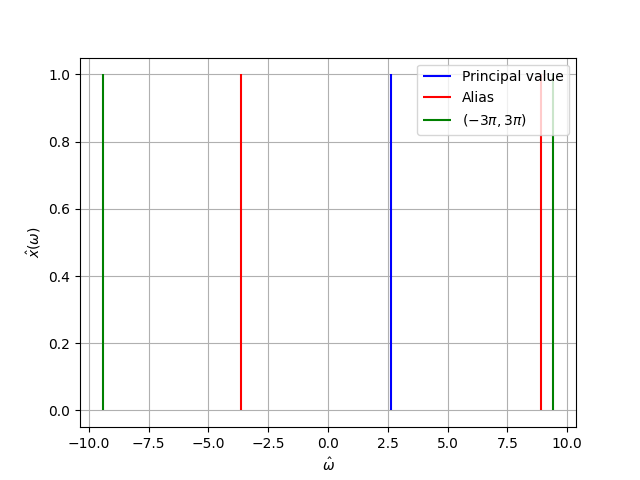
\includegraphics[width=\textwidth]{ch09/figures/spectrum_plot.png}
    \caption{Spectrum of $x(t)$, we see 3 spectral components in the range $(-3\pi,3\pi)$}
    \label{spectrum_plot}
\end{marginfigure}

\item The possible angular frequencies that result in the same discritization is found by
$$\omega_{k}=\omega_{0}+2\pi kf_{s}.$$
Choosing different values for $k$ to search for a value that satisfy the requirement of being the smallest $|\omega_{k}|$ is found to be $k=-100$. This value gives $\omega_{k}=2\pi42$. 

\item Here the signal is complex so the signal can be sampled at $f_{s}>f_{\text{max}}-f_{\text{min}}=\frac{\omega_{0}}{2\pi}$ by the Shannon which correspond to $f_{s}>10042$ Hz. 
\end{enumerate}

\item Given the continuous-time sinusoid $y_1[n] = 2 \cos(0.67 \pi n) + \cos(0.33 \pi n)$.
  \begin{enumerate}[a)]
    \item Using Euler's formula to first rewrite $y_{1}[n]$ on polar form:\\
    	\[y_1[n] = e^{i0.67\pi n} + e^{-i0.67\pi n} + \frac{1}{2}e^{i0.33\pi n} + \frac{1}{2}e^{-i0.33\pi n}\]
    	and then plot the spectrum (Figure \ref{fig:ex1}):\\
		\begin{marginfigure}
		  \begin{center}
			\begin{tikzpicture}
			  \begin{axis}[
			    width=7cm,height=6cm,ymin=0,ymax=1.3,xmin=-3.1,xmax=3.2,  
			    ytick={0.5,1}, yticklabels={,$1$}, 
			    xtick={-3,...,3},
			    xticklabels={$-3\pi$,$-2\pi$,$-\pi$,$0$,$\pi$,$2\pi$,$3\pi$}, 
			    ylabel={$y[n]$}, 
			    xlabel={$\hat{\omega}$}, axis lines = center]
			    
				\addplot+[ycomb,mark=*,mark color=skyblue1, solid,
						color=skyblue1] plot coordinates {(-2.6,1)(2.6,1)};
			  	\node at (axis cs:-2.67,1)[above,
			  				font={\footnotesize}]{$e^{-i2.67\pi}$};
			  	\node at (axis cs:2.67,1)[below,
			  				font={\footnotesize}]{$e^{i2.67\pi}$};
			  	
				\addplot+[ycomb,mark=*,mark color=scarletred1, solid,
						color=scarletred1] plot coordinates {(-2.33,0.5)(2.33,0.5)};
			  	\node at (axis cs:-2.33,0.5)[above,
			  				font={\footnotesize}]{$\frac{1}{2}e^{-i2.33\pi}$};
			  	\node at (axis cs:2.33,0.5)[below,
			  				font={\footnotesize}]{$\frac{1}{2}e^{i2.33\pi}$};
			  	
				\addplot+[ycomb,mark=*,mark color=scarletred1, solid,
						color=scarletred1] plot coordinates {(-1.67,0.5)(1.67,0.5)};
			  	\node at (axis cs:-1.67,0.5)[below,
			  				font={\footnotesize}]{$\frac{1}{2}e^{-i1.67\pi}$};
			  	\node at (axis cs:1.67,0.5)[above,
			  				font={\footnotesize}]{$\frac{1}{2}e^{i1.67\pi}$};
			  	
				\addplot+[ycomb,mark=*,mark color=skyblue1, solid,
						color=skyblue1] plot coordinates {(-1.33,1)(1.33,1)};
			  	\node at (axis cs:-1.33,1)[below,
			  				font={\footnotesize}]{$e^{-i0.33\pi}$};
			  	\node at (axis cs:1.33,1)[above,
			  				font={\footnotesize}]{$e^{i0.33\pi}$};
			  	
			  	\addplot+[ycomb,mark=*,mark color=blue, solid,
						color=blue] plot coordinates {(-0.67,1)(0.67,1)};
			  	\node at (axis cs:-0.67,1)[above,
			  				font={\footnotesize}]{$e^{-i0.67\pi}$};
			  	\node at (axis cs:0.67,1)[below,
			  				font={\footnotesize}]{$e^{i0.67\pi}$};
			  	
				\addplot+[ycomb,mark=*,mark color=red, solid,
						color=red] plot coordinates {(-0.33,0.5)(0.33,0.5)};
			  	\node at (axis cs:-0.33,0.5)[above,
			  				font={\footnotesize}]{$\frac{1}{2}e^{-i0.33\pi}$};
			  	\node at (axis cs:0.33,0.5)[below,
			  				font={\footnotesize}]{$\frac{1}{2}e^{i0.33\pi}$};
			  	
			  \end{axis}
			\end{tikzpicture}
		  \end{center}
		\caption{Spectrum for 1.a): \\ $y_1[n] = 2 \cos(0.67 \pi n) + \cos(0.33 \pi n)$ \\ Shown only frequency components from principal up to 2nd alias.}
		\label{fig:ex1}
		\end{marginfigure}
    
    \item For the changed signal $y_2[n] = 2 \cos(2.67 \pi n) + \cos(0.33 \pi n)$, the spectrum will stay unchanged because $\cos(2.67 \pi n) = \cos(0.67 \pi n)$.
  \end{enumerate}
  
\item A sampling rate of 24 fps equals 1440 frames per minute.
\begin{enumerate}[a)]
    \item When the disc speed equals the camera's sampling rate at 1440 rpm, the red spot will be recorded at the same position for every frame, and thus appears to be standing still.
    \item When the disc speed gets larger than the Shannon-Nyquist sampling theorem, $v_{rot} > f_s / 2 > 720$ rpm, aliasing starts to occur. Within the speed range of $720 < v_{rot} < 1440$ rpm, the phase of the alias has the opposite sign than the phase of the real rotation, and so the red spot seems to rotate counter-clockwise with decreasing speed as $v_{rot}$ increases.
    \item Aliasing in the interval with opposite phase sign is called \emph{folding}.
    \item When $1440 < v_{rot} < 2880$, there is no folding, and the corresponding alias of the red spot will have speed $0 < v_{rot} < 1440$ rpm.
\end{enumerate}

\item Let $x(t)=(2\pi)^{-1}\int_{-\infty}^{\infty}\hat{x}(\omega)e^{i\omega t}d\omega$.

\begin{enumerate}[a)]
\item By the definition of $|\hat{x}(\omega)|$ and the Figure we see that there is no pairing for the frequencies, meaning that $\hat{x}^{*}(\omega)\neq \hat{x}(-\omega)$, so $x(t)$ can't be real.

\item For complex signals we must sample at a rate that satisfy $f_{s}>f_{\text{max}}-f_{\text{min}}=\frac{1}{2\pi}(\omega_{1}-\omega_{0})$ in units of Hz. 

\item By the Shannon–sampling theorem the sample-rate $f_{s}$ from above is sufficient to retain all the information regarding the signal, thus the spectrum has no overlap. This is reflected in the drawing of $|\hat{x}_{s}(\omega)|$ where the copies are shown in red.

\begin{center}
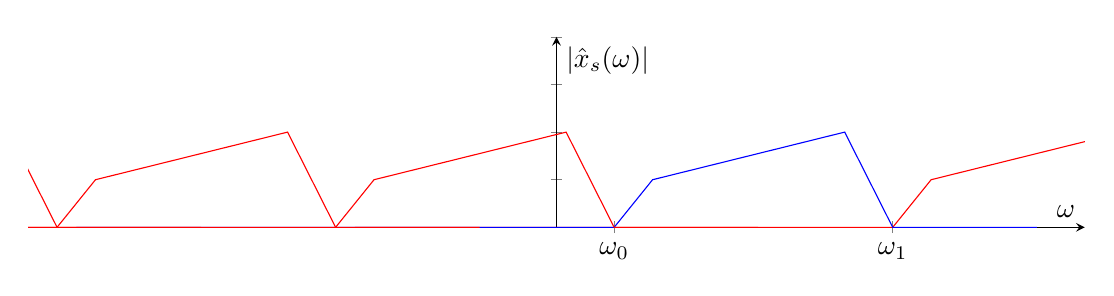
\begin{tikzpicture}
\begin{axis}[width=15cm,height=4cm,ymin=0,ymax=2,
    	xmin=-11,xmax=11,
        xlabel={$\omega$},
        ylabel={$|\hat{x}_{s}(\omega)|$},
        axis x line=center, 
        axis y line=center, 
        yticklabels={,,,},
        xtick={1.2,7},
        xticklabels={$\omega_0$,$\omega_1$}
    ]
    \addplot[mark=none,color=red] plot coordinates {(-4.2,0) (7.0,0) (7.8,0.5) (11.8,1) (12.8,0) (15.8,0)};
    \addplot[mark=none,color=blue] plot coordinates {(-10,0) (1.2,0) (2,0.5) (6,1) (7,0) (10,0)};
    \addplot[mark=none,color=red] plot coordinates {(-15.8,0) (-4.6,0) (-3.8,0.5) (0.2,1) (1.2,0) (4.2,0)};
    \addplot[mark=none,color=red] plot coordinates {(-21.6,0) (-10.4,0) (-9.6,0.5) (-5.6,1) (-4.6,0) (-1.6,0)};
    \addplot[mark=none,color=red] plot coordinates {(-27.4,0) (-16.2,0) (-15.4,0.5) (-11.4,1) (-10.4,0) (-7.4,0)};
\end{axis}
\end{tikzpicture}
\end{center}

\item In this case, the reconstruction filter would be an ideal band-pass filter of the form
$$\mathcal{H}(\omega)=\begin{cases}
    T_{s}, \quad \omega_{1}\le\omega\le\omega_{2}, \\
    0, \quad \hspace{0.1cm}\text{otherwise}.
\end{cases}$$
Have $x_{s}(t)$ as
$$x_{s}(t)=\sum_{n=-\infty}^{\infty}x[n]\delta(t-nT_{s}),$$
from the samples. To reconstruct the signal simply multiply $\hat{x}(\omega)$ by the reconstruction filter in frequency domain. The frequency domain representation of $x_{s}(t)$ was shown to be
$$\hat{x}_{s}(\omega)=\frac{1}{T_{s}}\sum_{n=-\infty}^{\infty}\hat{x}(\omega-n\omega_{s}).$$
Where $\omega_{s}=2\pi f_{s}$. Thus, multiplying in frequency domain yields
$$\mathcal{H}(\omega)\hat{x}_{s}(\omega)=T_{s}\frac{1}{T_{s}}\sum_{n=-\infty}^{\infty}\hat{x}(\omega-n\omega_{s})=\hat{x}(\omega),$$
here the sum is killed by $\mathcal{H}(\omega)$ as it is $0$ outside of $\omega_{1}\le\omega\le\omega_{2}$. Hence we retain all the information necessary to reconstruct the signal as 
$$x(t)=(2\pi)^{-1}\int_{-\infty}^{\infty}\hat{x}(\omega)e^{i\omega t}d\omega.$$
\end{enumerate}



\item As before let $x(t)=(2\pi)^{-1}\int_{-\infty}^{\infty}\hat{x}(\omega)e^{i\omega t}d\omega$ and
$$|\hat{x}(\omega)|=\begin{cases}
    > 0 \quad    \text{when} \quad \omega_{0}<|\omega|<\omega_{1},\\
    0, \quad     \text{otherwise},
\end{cases}$$
with $\omega_{0}=2\pi30$ and $\omega_{1}=2\pi40$ radians per second. Here we use a sample rate of $f_{s}=20$ Hz or $\omega_{s}=2\pi 20$ radians per sample. 

\begin{enumerate}[a)]
\item We know that $\hat{x}(\omega)=\hat{x}^{*}(-\omega)$ so the signal is real-valued. 

\item Draw $|\hat{x}_{s}(\omega)|$ with the different aliases shown in red:
\begin{center}
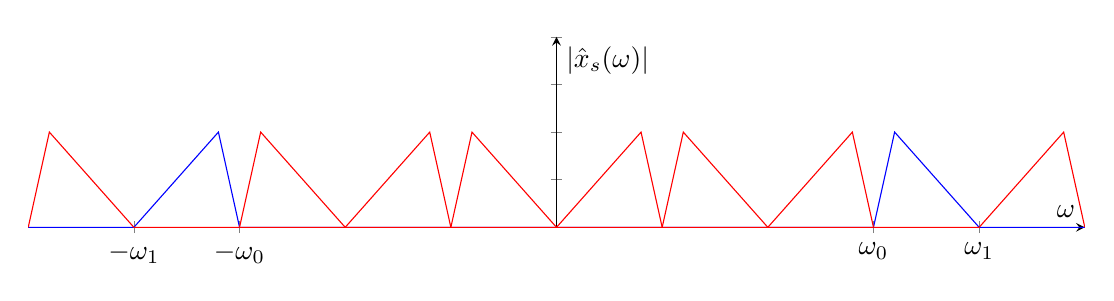
\begin{tikzpicture}
	\begin{axis}[width=15cm,height=4cm,ymin=0,ymax=2,
    	xmin=-50,xmax=50,
        xlabel={$\omega$},
        ylabel={$|\hat{x}_{s}(\omega)|$},
        axis x line=center, 
        axis y line=center, 
        yticklabels={,,,},
        xtick={-40,-30,30,40},
        xticklabels={$-\omega_1$,$-\omega_0$,$\omega_0$,$\omega_1$}
    ]
    \addplot[mark=none,color=blue] plot coordinates {(-50,0) (-40,0) (-32,1) (-30,0) (30,0) (32,1) (40,0) (50,0)};
    \addplot[mark=none,color=red] plot coordinates {(10,0) (12,1) (20,0) (30,0)};
    \addplot[mark=none,color=red] plot coordinates {(-10,0) (-8,1) (0,0) (10,0)};
    \addplot[mark=none,color=red] plot coordinates {(-30,0) (-28,1) (-20,0) (-10,0)};
    \addplot[mark=none,color=red] plot coordinates {(-50,0) (-48,1) (-40,0) (-30,0)};
    \addplot[mark=none,color=red] plot coordinates {(-30,0) (-20,0) (-12,1) (-10,0)};
    \addplot[mark=none,color=red] plot coordinates {(-10,0) (0,0) (8,1) (10,0)};
    \addplot[mark=none,color=red] plot coordinates {(10,0) (20,0) (28,1) (30,0)};
    \addplot[mark=none,color=red] plot coordinates {(30,0) (40,0) (48,1) (50,0)};
\end{axis}
\end{tikzpicture}
\end{center}

\item The condition $f_{s}>2f_{\text{max}}$ is violated in this case. This condition applies to real signals but assumes the frequencies fall in the principal spectrum of $|f|<f_{s}/2$ which is not the case here. However, the sample rate satisfy
$$n\frac{\omega_{s}}{2}\le|\omega|\le(n+1)\frac{\omega_{s}}{2}$$
or
$$n2\pi 10\le|\omega|\le (n+1)2\pi10$$
which is satisfied for $n=3$, as this gives
$$2\pi 30\le |\omega|\le 2\pi 40$$
this bounds the spectrum and avoids aliasing, hence this is sufficient to retain all the information in the signal. 

\item Define a filter $\mathcal{H}(\omega)$ as an ideal band-pass filter
$$\mathcal{H}(\omega)=\begin{cases}
    T_{s}, \quad \omega_{0}\le|\omega|\le\omega_{1}, \\
    0, \quad \hspace{0.1cm}\text{otherwise}.
\end{cases}$$
then 
$$\mathcal{H}(\omega)\hat{x}_{s}(\omega)=T_{s}\frac{1}{T_{s}}\sum_{k=-\infty}^{\infty}\hat{x}(\omega-k\omega_{s})=\hat{x}(\omega).$$
Due to $\mathcal{H}(\omega)$ being $0$ outside $\omega_{0}\le|\omega|\le\omega_{1}$ the sum goes away giving back the original frequency representation of the signal. Note that the absolute value is needed here to get both the positive and negative frequencies as the signal is real, then applying the Fourier transform to this signal yields the original signal $x(t)$. 
\end{enumerate}

















\end{enumerate}
